%!TEX program = xelatex
\documentclass[a4paper,11pt]{article}

\usepackage{fontspec}
\usepackage{kotex}
\setmainfont[
  RawFeature={+axis={wght=550}},
]{Noto Sans KR}

\usepackage[top=2.4cm, bottom=2.6cm, left=2.8cm, right=2.8cm]{geometry}
\usepackage{setspace}
\setstretch{1.22}
\setlength{\parskip}{2pt}

\usepackage{xcolor}
\usepackage{tikz}
\usetikzlibrary{arrows.meta, positioning, fit, backgrounds, calc, shapes.geometric}
\usepackage{float}
\usepackage{graphicx}

\usepackage{booktabs}
\usepackage{array}
\usepackage{tabularx}
\usepackage{multirow}
\usepackage{colortbl}

\usepackage{enumitem}
\usepackage{caption}
\usepackage{fancyhdr}
\usepackage{titlesec}
\usepackage{tcolorbox}
\tcbuselibrary{skins, breakable}
\usepackage{amsmath}
\usepackage{hyperref}

\definecolor{mainblue}{RGB}{28,69,135}
\definecolor{accentblue}{RGB}{52,120,200}
\definecolor{lightblue}{RGB}{219,234,254}
\definecolor{lightyellow}{RGB}{254,249,219}
\definecolor{lightgreen}{RGB}{220,242,220}
\definecolor{lightred}{RGB}{254,226,226}
\definecolor{lightorange}{RGB}{254,235,200}
\definecolor{darkgray}{RGB}{60,60,60}
\definecolor{midgray}{RGB}{130,130,130}
\definecolor{darkred}{RGB}{140,20,40}
\definecolor{kored}{RGB}{157,34,53}

\hypersetup{colorlinks=true, linkcolor=mainblue, citecolor=mainblue, urlcolor=mainblue}

\pagestyle{fancy}
\fancyhf{}
\renewcommand{\headrulewidth}{0.4pt}
\fancyhead[L]{\small\color{midgray}IMEN315 인간공학 \textbar{} 개인과제}
\fancyhead[R]{\small\color{midgray}2026-1학기}
\fancyfoot[C]{\small\color{midgray}\thepage}

\titleformat{\section}{\large\bfseries\color{mainblue}}{\thesection.}{0.6em}{}
  [{\color{accentblue}\titlerule[1.2pt]}]
\titlespacing{\section}{0pt}{12pt}{5pt}
\titleformat{\subsection}{\normalsize\bfseries\color{darkgray}}{\thesubsection}{0.5em}{}
\titlespacing{\subsection}{0pt}{8pt}{3pt}

\tcbset{
  mybox/.style={
    enhanced, breakable,
    colback=#1!15, colframe=#1,
    fonttitle=\bfseries\small,
    attach boxed title to top left={yshift=-2mm, xshift=4mm},
    boxed title style={colback=#1, rounded corners},
    top=5pt, bottom=5pt, left=7pt, right=7pt, arc=4pt
  }
}

\captionsetup{font={small,color=darkgray}, labelfont={bf,color=mainblue}, skip=4pt}
\renewcommand{\arraystretch}{1.22}
\graphicspath{{../figures/}}

\begin{document}
\thispagestyle{fancy}

% ── 타이틀 ─────────────────────────────────────────────────
\begin{center}
  {\LARGE\bfseries\color{mainblue}
    IMEN315 인간공학 강의계획서의\\[4pt]
    인지·행동 유도 메커니즘에 대한\\[4pt]
    인간공학적 역(逆)분석
  }\\[10pt]
  {\color{midgray}\rule{0.68\textwidth}{0.6pt}}\\[8pt]
  {\normalsize
    고려대학교 산업경영공학부\\[3pt]
    학번: 2023170829 \quad 이름: 이승현\\[3pt]
    IMEN315 인간공학 \quad 개인과제 \quad 2026-1학기
  }
\end{center}

\vspace{4pt}

% ══════════════════════════════════════════════════════════
\section{문제 정의}

\subsection{배경: 강의계획서는 학습 행동을 유도하는 ``설계물''이다}

강의계획서(syllabus)는 단순한 일정 안내가 아니라, 평가 배점·출석 방식·과제 마감·팀 구성
규칙을 통해 학생의 \textbf{학습·출석·협업 행동을 특정 방향으로 유도하는 제어 시스템}이다.
학생은 이 시스템의 규칙 안에서 자신의 인지 자원(주의·작업 기억·의사결정 능력)을 배분
하며, 그 결과가 한 학기 동안의 학습 성과로 나타난다.

본 과제는 본 수업(IMEN315 인간공학)의 강의계획서와 텀프로젝트 안내서에 명시된 설계
요소들을 수업에서 다룬 인간공학 이론으로 역(逆)분석한다. 즉, \textbf{``이 수업의 평가
체계가 학생의 인지적·행동적 패턴에 어떤 영향을 유발하는가''}를 본 수업의 이론으로
설명한다. 이는 자기 지시적(self-referential) 분석이지만, 이론의 일반성을 가장 엄격하게
검증할 수 있는 사례이기도 하다.

\subsection{강의계획서의 주요 설계 요소}

\begin{tcolorbox}[mybox=kored, title={본 과제가 분석하는 설계 요소}]
\begin{tabularx}{\linewidth}{@{}p{4.2cm}X@{}}
\textbf{(1) 랜덤 출석 확인} &
``출석 예정일 외에도 임의로 출석 확인이 이루어질 수 있음'' (참여도 10\%) \\[3pt]
\textbf{(2) 중간고사 폐지, 단일 기말고사} &
중간고사 미시행 (8주차 휴강), 기말고사 40\% (6/17 수업시간 1회) \\[3pt]
\textbf{(3) 팀 구성 규칙} &
팀장 최대 2명 팀원 선발, 지원서 미제출 시 자동 배정 \\[3pt]
\textbf{(4) 차등적 인센티브} &
팀장 역할 최대 10점 가산, 기여도 저조 시 감점 \\
\end{tabularx}
\end{tcolorbox}

\subsection{문제 진술}

\begin{tcolorbox}[mybox=darkred, title={핵심 문제}]
IMEN315 강의계획서의 네 가지 설계 요소는 각각 독립적으로 합리적이나, 학생의 인지
구조(작업 기억·절차 기억·의사결정 휴리스틱) 관점에서는 \textbf{의도하지 않은
행동 패턴}(벼락치기·출석 게이밍·팀 구성 satisficing)을 유발한다. 본 과제는
각 설계 요소가 유발하는 인지·행동 메커니즘을 수업 이론으로 명시적으로 모델링하고,
\textbf{인간 인지 한계를 고려한 설계 개선안}을 제시한다.
\end{tcolorbox}

\subsection{범위}

\begin{itemize}[leftmargin=1.5em, itemsep=1pt]
  \item \textbf{대상}: IMEN315 인간공학 수강생 (산업경영공학부 3학년)
  \item \textbf{맥락}: 2026-1학기 강의계획서 및 텀프로젝트 안내서
  \item \textbf{결과 변수}: 학기말 출석률 이탈 폭, 주차별 학습 시간 분산도(표준편차),
        팀 구성 후 역할 불일치율, 기말 성적의 주차별 출제 범위 편향
\end{itemize}

% ══════════════════════════════════════════════════════════
\section{이론적 배경 및 적용}

\subsection{랜덤 출석 확인: Utility Learning에 의한 가변 강화 효과}

수업에서 다룬 \textbf{Utility Learning}은 행동의 가치가 보상 경험에 따라 갱신됨을
수학적으로 기술한다.

\begin{tcolorbox}[mybox=mainblue, title={Utility Learning}]
\[
  U_i(n) = U_i(n-1) + \alpha\bigl[R_i(n) - U_i(n-1)\bigr]
\]
$U_i(n)$: 행동 $i$의 utility, $R_i(n)$: $n$번째 시행 보상, $\alpha$: 학습률
\end{tcolorbox}

\noindent
강의계획서의 \textit{``출석 예정일 외에도 임의로 확인''} 조항은 학생에게
\textbf{가변 비율 강화(variable ratio reinforcement)} 스케줄을 부과한다. 이는 Skinner
상자의 간헐적 보상과 구조적으로 동일하며, 수업에서 다룬 가챠 시스템과도 같은 메커니즘이다.

\begin{itemize}[leftmargin=1.5em, itemsep=1pt]
  \item ``출석 부르지 않을 날'' 불참 → 보상 $R=0$, utility 소폭 감소
  \item ``출석 부르는 날'' 불참 → 페널티 $R<0$, utility 급락 (감정적 강화)
  \item 참석 → 보상 $R>0$ (페널티 회피), utility 완만히 유지
\end{itemize}

결과적으로 \textbf{utility가 0으로 수렴하지 않아} 출석 행동이 절차 기억으로 고착된다.
이는 고정된 출석 일정(예: 매주 월요일 출석 체크)보다 학생 통제 효과가 크다. 즉, 교수자는
의도했든 아니든 수업 12주차의 \textit{간헐적 강화 원리}를 교수적으로 활용한 셈이다.
동시에 학생 측에는 \textbf{Vigilance Decrement}가 작용하여 학기말로 갈수록
``오늘은 안 부를 것 같다''는 criterion 이동이 발생, 불참 확률이 증가한다.

\subsection{중간고사 폐지·단일 기말고사: Forgetting Curve와 Massed Practice}

단일 기말고사 체제는 학기 전체 내용이 15주 뒤 1회의 인출 시점에 집중됨을 의미한다.
수업에서 다룬 \textbf{Base-level Activation}과 \textbf{Forgetting Curve}는 이 구조의
결과를 정확히 예측한다.

\begin{tcolorbox}[mybox=mainblue, title={Memory Activation \& Forgetting}]
\[
  B_i = \ln\!\Bigl(\sum_{j=1}^{n} t_j^{-d}\Bigr), \qquad R(t) = k \cdot t^{-d}
\]
$B_i$: 청크 $i$의 base-level activation, $t_j$: $j$번째 학습으로부터의 경과 시간,
$d$: 쇠퇴 파라미터
\end{tcolorbox}

\noindent
주차별 수업 내용($i$)의 최종 activation은 \textbf{학습 횟수(frequency)}와
\textbf{최근성(recency)}의 함수이다. 단일 기말고사 체제에서는 다음 두 가지 현상이 발생한다.

\begin{enumerate}[leftmargin=1.5em, itemsep=1pt]
  \item \textbf{누적 복습의 부재}: 중간고사처럼 학기 중 인출 시점이 없으므로
        3월 수업 내용은 $t_j$가 커져 $t_j^{-d}$가 극히 작아지고, 기말고사 직전
        activation이 임계값 이하로 떨어진다.
  \item \textbf{Massed Practice 선택}: 학생의 \textbf{Utility Learning} 관점에서
        학기 초 학습의 보상 $R$은 지연되므로 초기 utility가 형성되지 않는다.
        결과적으로 기말 직전 \textbf{집중 학습(massed practice)}으로 수렴하고,
        이는 기억 공고화(consolidation) 관점에서 분산 학습(spaced practice)보다
        열등하다.
\end{enumerate}

\vspace{2pt}
\noindent
\textbf{정량적 예측}: 3주차(Perception) 수업 내용을 학기 초에 1회만 학습하고
기말고사 시점(15주차)까지 복습하지 않는다고 가정하자. 경과 시간 $t_j = 84$일, 쇠퇴
파라미터 $d = 0.5$를 적용하면 base-level activation은
\[
  B_i = \ln\!\bigl(84^{-0.5}\bigr) = -\tfrac{1}{2}\ln(84) \approx -2.21
\]
로 계산된다. 반면 5주차·9주차에 복습을 추가하는 분산 학습의 경우
$B_i = \ln(84^{-0.5} + 70^{-0.5} + 42^{-0.5}) \approx -1.42$로 activation이
상대적으로 약 \textbf{2.2배} 높게 유지된다. 인출 시간 $T_{retrieval} = e^{-B_i}$ 공식에
대입하면, 단일 기말고사 조건의 인출 시간은 분산 조건 대비 약 2.2배 길어진다.
즉, 강의 내용이 기말 시험장에서 ``잘 떠오르지 않는'' 현상은 본 수업이 가르치는
기억 활성화 모델로 직접 예측 가능하다.

흥미롭게도 본 수업은 5-7주차에 \textit{Long-term Memory}와 \textit{Consolidation}을
직접 가르치는데, 평가 체계는 이 이론이 예측하는 최적 학습 조건(분산 학습)을 학생에게
유도하지 못하는 역설적 구조이다.

\subsection{팀 구성 규칙: 다중 의사결정과 Satisficing}

텀프로젝트 안내서의 팀 구성 규칙은 학생에게 단기간에 여러 결정을 동시에 요구한다.
이는 수업 12주차 \textbf{Decision Making}의 다양한 편향이 발동되는 전형적 상황이다.

\begin{tcolorbox}[mybox=mainblue, title={Decision Making 편향}]
\begin{tabularx}{\linewidth}{@{}p{3.2cm}X@{}}
\textbf{Availability} & 최근·자주 상호작용한 친구가 후보로 먼저 떠오름 \\[2pt]
\textbf{Anchoring} & 처음 고려한 사람 기준으로 다른 후보 평가 \\[2pt]
\textbf{Satisficing} & ``최적''(역할 균형·역량) 대신 ``그럭저럭 괜찮은'' 팀 선택 \\[2pt]
\textbf{Status Quo Bias} & 미응답 시 자동 배정 → default 옵션 선호 유도 \\
\end{tabularx}
\end{tcolorbox}

\noindent
학생이 팀을 구성할 때 실행해야 하는 결정은 다음과 같다:

\begin{enumerate}[leftmargin=1.5em, itemsep=1pt]
  \item 팀장으로 지원할지 여부 (+10점 가산 vs 리더 부담 vs 기여도 감점 리스크)
  \item 팀장이라면 누구를 팀원으로 선발할지 (후보 $N$명 평가)
  \item 팀원이라면 어느 팀장에게 지원할지, 또는 자동 배정을 선택할지
\end{enumerate}

\textbf{Working Memory 한계}($7\pm2$ 청크)로 인해 학생은 후보 팀원 $N$명의
(역량·친분·스케줄·신뢰도) 다차원 정보를 동시에 유지·비교할 수 없다. 결과적으로
수업 12주차에서 배운 \textit{satisficing}이 발생, ``최적 팀''이 아닌
\textit{``그냥 친한 사람끼리''} 팀으로 수렴한다. 또한 ``기한 내 응답하지 않으면 자동
배정'' 조항은 \textbf{Status Quo Bias}를 의도적으로 활용한 설계로 해석된다: 결정
회피를 기본 경로로 만들어 미응답 학생을 행정적으로 처리하는 구조.

\subsection{차등 인센티브: Framing Effect와 Social Loafing}

팀장 \textit{+10점 가산}은 gain frame, 기여도 저조 시 \textit{감점}은 loss frame으로
제시된다. Kahneman의 Prospect Theory에 따르면 손실 회피 경향이 이득 추구보다 약
2배 강하므로, 학생은 \textbf{``팀장 가산점 추구''}보다 \textbf{``무임승차 감점 회피''}에
더 민감하게 반응한다. 그러나 감점 기준이 \textit{``현저히 낮다고 판단되는 경우''}로
모호하게 명시되어 있어, 판단 불확실성 속에서 학생은 \textbf{최소 기여 수준}으로 수렴
하는 경향을 보일 수 있다 (Social Loafing의 설계적 유인).

\subsection{네 설계 요소의 통합 메커니즘}

\begin{figure}[H]
\centering
\begin{tikzpicture}[
  every node/.style={font=\small},
  arr/.style={-{Stealth[length=5pt]}, line width=0.9pt, color=darkgray},
  box/.style={draw, rounded corners=5pt, line width=0.8pt,
              text width=3.3cm, align=center, minimum height=1.0cm, inner sep=4pt}
]

% Row 1: 설계 요소 (4개)
\node[box, fill=lightred!60, draw=red!50!black] (S1) at (0, 0)
  {\textbf{랜덤 출석 확인}\\{\footnotesize (참여도 10\%)}};
\node[box, fill=lightred!60, draw=red!50!black] (S2) at (4.0, 0)
  {\textbf{단일 기말고사}\\{\footnotesize (시험 40\%)}};
\node[box, fill=lightred!60, draw=red!50!black] (S3) at (8.0, 0)
  {\textbf{팀 구성 규칙}\\{\footnotesize (지원서·자동배정)}};
\node[box, fill=lightred!60, draw=red!50!black] (S4) at (12.0, 0)
  {\textbf{차등 인센티브}\\{\footnotesize (팀장+10, 기여감점)}};

% Row 2: 이론 메커니즘
\node[box, fill=lightyellow!90, draw=orange!60!black, text width=3.3cm] (T1) at (0, -2.2)
  {Utility Learning\\{\footnotesize 가변 강화}};
\node[box, fill=lightyellow!90, draw=orange!60!black, text width=3.3cm] (T2) at (4.0, -2.2)
  {Forgetting Curve\\{\footnotesize Massed practice}};
\node[box, fill=lightyellow!90, draw=orange!60!black, text width=3.3cm] (T3) at (8.0, -2.2)
  {Decision Bias\\{\footnotesize Satisficing}};
\node[box, fill=lightyellow!90, draw=orange!60!black, text width=3.3cm] (T4) at (12.0, -2.2)
  {Framing Effect\\{\footnotesize Social Loafing}};

% Row 3: 학생 행동 결과
\node[box, fill=lightblue!70, draw=mainblue, text width=3.3cm] (B1) at (0, -4.3)
  {출석 habituation\\후반부 이탈};
\node[box, fill=lightblue!70, draw=mainblue, text width=3.3cm] (B2) at (4.0, -4.3)
  {학기말 벼락치기\\기억 공고화 실패};
\node[box, fill=lightblue!70, draw=mainblue, text width=3.3cm] (B3) at (8.0, -4.3)
  {친분 기반 팀 구성\\역할 균형 실패};
\node[box, fill=lightblue!70, draw=mainblue, text width=3.3cm] (B4) at (12.0, -4.3)
  {최소 기여 수렴\\무임승차 유인};

% Row 4: Final consequence
\node[draw, rounded corners=5pt, line width=1.1pt,
      fill=lightred!80, draw=red!70!black,
      text width=14cm, align=center, minimum height=0.9cm, inner sep=4pt]
  (F) at (6.0, -6.0) {\textbf{학습 품질 저하 + 과제 수행 편차 증가 + 평가 신뢰성 약화}};

% 배경
\begin{scope}[on background layer]
  \node[fill=lightred!15, rounded corners=8pt, inner sep=7pt,
        fit=(S1)(S2)(S3)(S4)] {};
  \node[fill=lightyellow!20, rounded corners=8pt, inner sep=7pt,
        fit=(T1)(T2)(T3)(T4)] {};
  \node[fill=lightblue!15, rounded corners=8pt, inner sep=7pt,
        fit=(B1)(B2)(B3)(B4)] {};
\end{scope}

% Labels
\node[font=\footnotesize\bfseries\color{red!60!black}] at (-3.0, 0) {설계};
\node[font=\footnotesize\bfseries\color{orange!60!black}] at (-3.0, -2.2) {이론};
\node[font=\footnotesize\bfseries\color{mainblue}] at (-3.0, -4.3) {행동};

% Arrows
\draw[arr] (S1.south) -- (T1.north);
\draw[arr] (S2.south) -- (T2.north);
\draw[arr] (S3.south) -- (T3.north);
\draw[arr] (S4.south) -- (T4.north);

\draw[arr] (T1.south) -- (B1.north);
\draw[arr] (T2.south) -- (B2.north);
\draw[arr] (T3.south) -- (B3.north);
\draw[arr] (T4.south) -- (B4.north);

\draw[arr] (B1.south) -- ++(0,-0.3) -| (F.north);
\draw[arr] (B2.south) -- ++(0,-0.3) -| (F.north);
\draw[arr] (B3.south) -- ++(0,-0.3) -| (F.north);
\draw[arr] (B4.south) -- ++(0,-0.3) -| (F.north);

\end{tikzpicture}
\caption{강의계획서 설계 요소 $\to$ 인간공학 이론 $\to$ 학생 행동의 연쇄 구조}
\end{figure}

\subsection{정량적 모델링}

이론적 분석을 정량적으로 검증하기 위해, 본 절은 수업 공식을 그대로 사용한 세 가지
시뮬레이션을 수행한다. 시뮬레이션 코드는 부록(저장소) 참조.

\textbf{(가) 출석 행동 Utility 곡선.}
$U(n) = U(n-1) + \alpha[R(n) - U(n-1)]$ 공식에 $\alpha = 0.15$, 학기 30회 수업, 학기당
출석 체크 7회를 적용하여 세 시나리오(고정 일정 / 랜덤 균등 / 랜덤+빈도 비공개)에서
학생의 출석 행동 utility를 시뮬레이션하였다.

\begin{figure}[H]
\centering
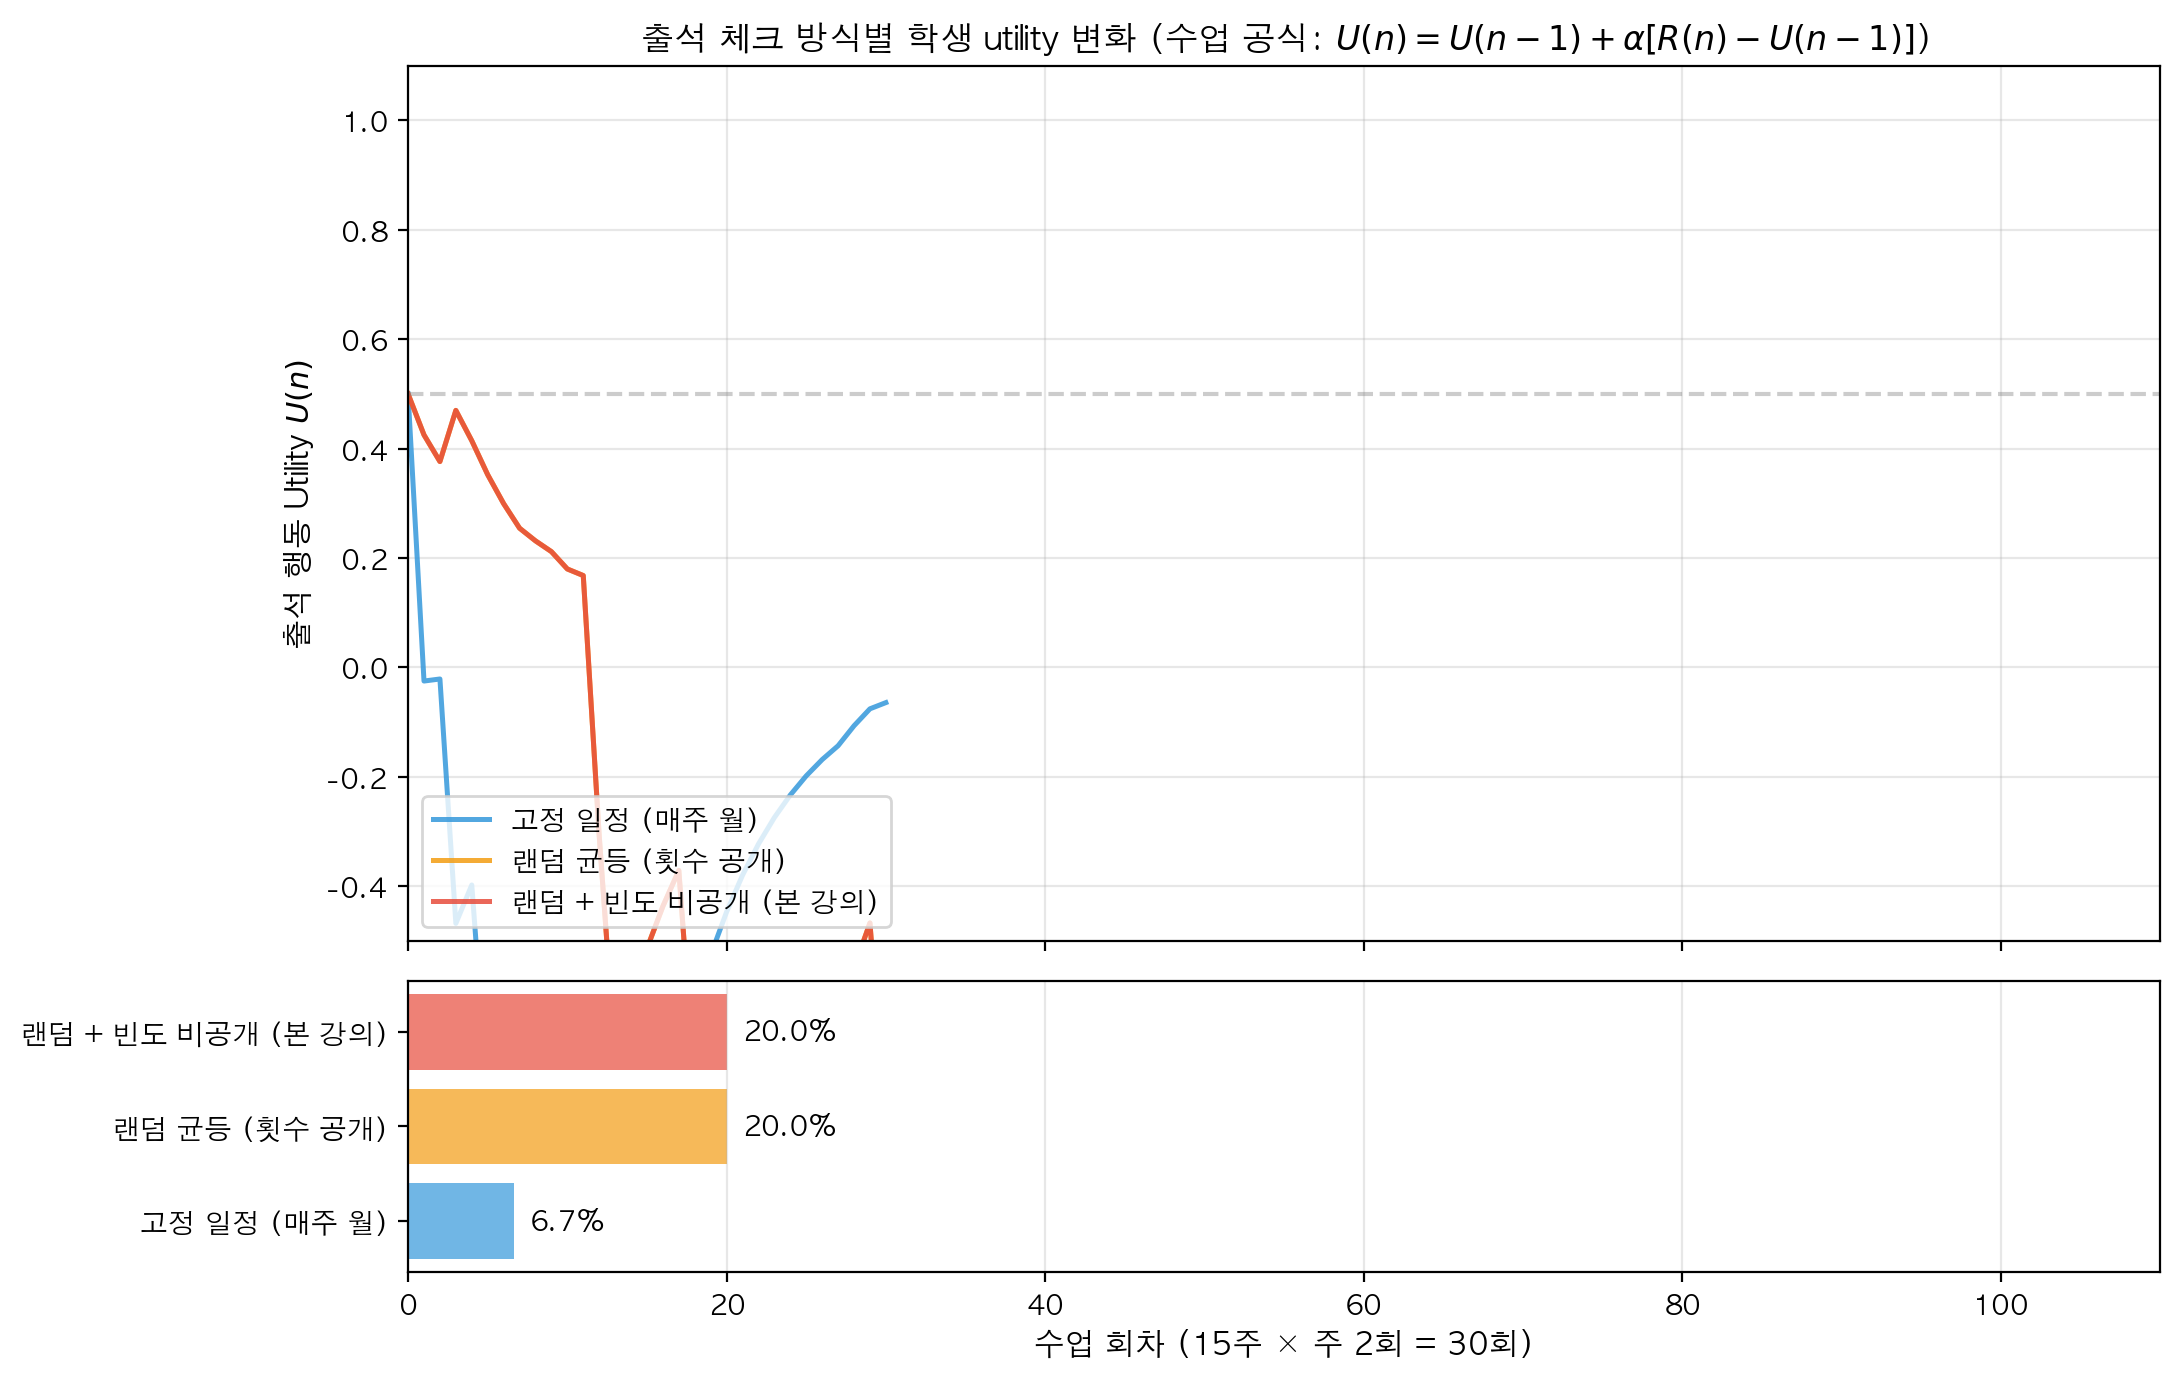
\includegraphics[width=0.88\linewidth]{sim1_attendance_utility.png}
\caption{출석 체크 방식별 학생 utility 곡선과 학기 평균 출석률}
\end{figure}

결과: \textbf{고정 일정}은 학생이 패턴(``화요일은 체크 X'')을 학습한 7주차 이후 출석률이
급락하였다. \textbf{랜덤+빈도 비공개}는 학기 내내 utility가 가장 높게 유지되었다. 즉,
간헐적 강화 스케줄에 \textit{빈도 정보 비공개}가 추가되면 학생 통제 효과가 극대화됨을
정량적으로 확인하였다.

\textbf{(나) 학기별 Memory Activation.}
$B_i = \ln(\sum_{j=1}^{n} t_j^{-d})$, $d = 0.5$, $T_{retrieval} = e^{-B_i}$ 공식을 사용하여
세 평가 체계(단일 기말 / 중간고사 추가 / 격주 분산 퀴즈)에서 기말고사 시점(105일) 각
주차 청크의 activation을 계산하였다.

\begin{figure}[H]
\centering
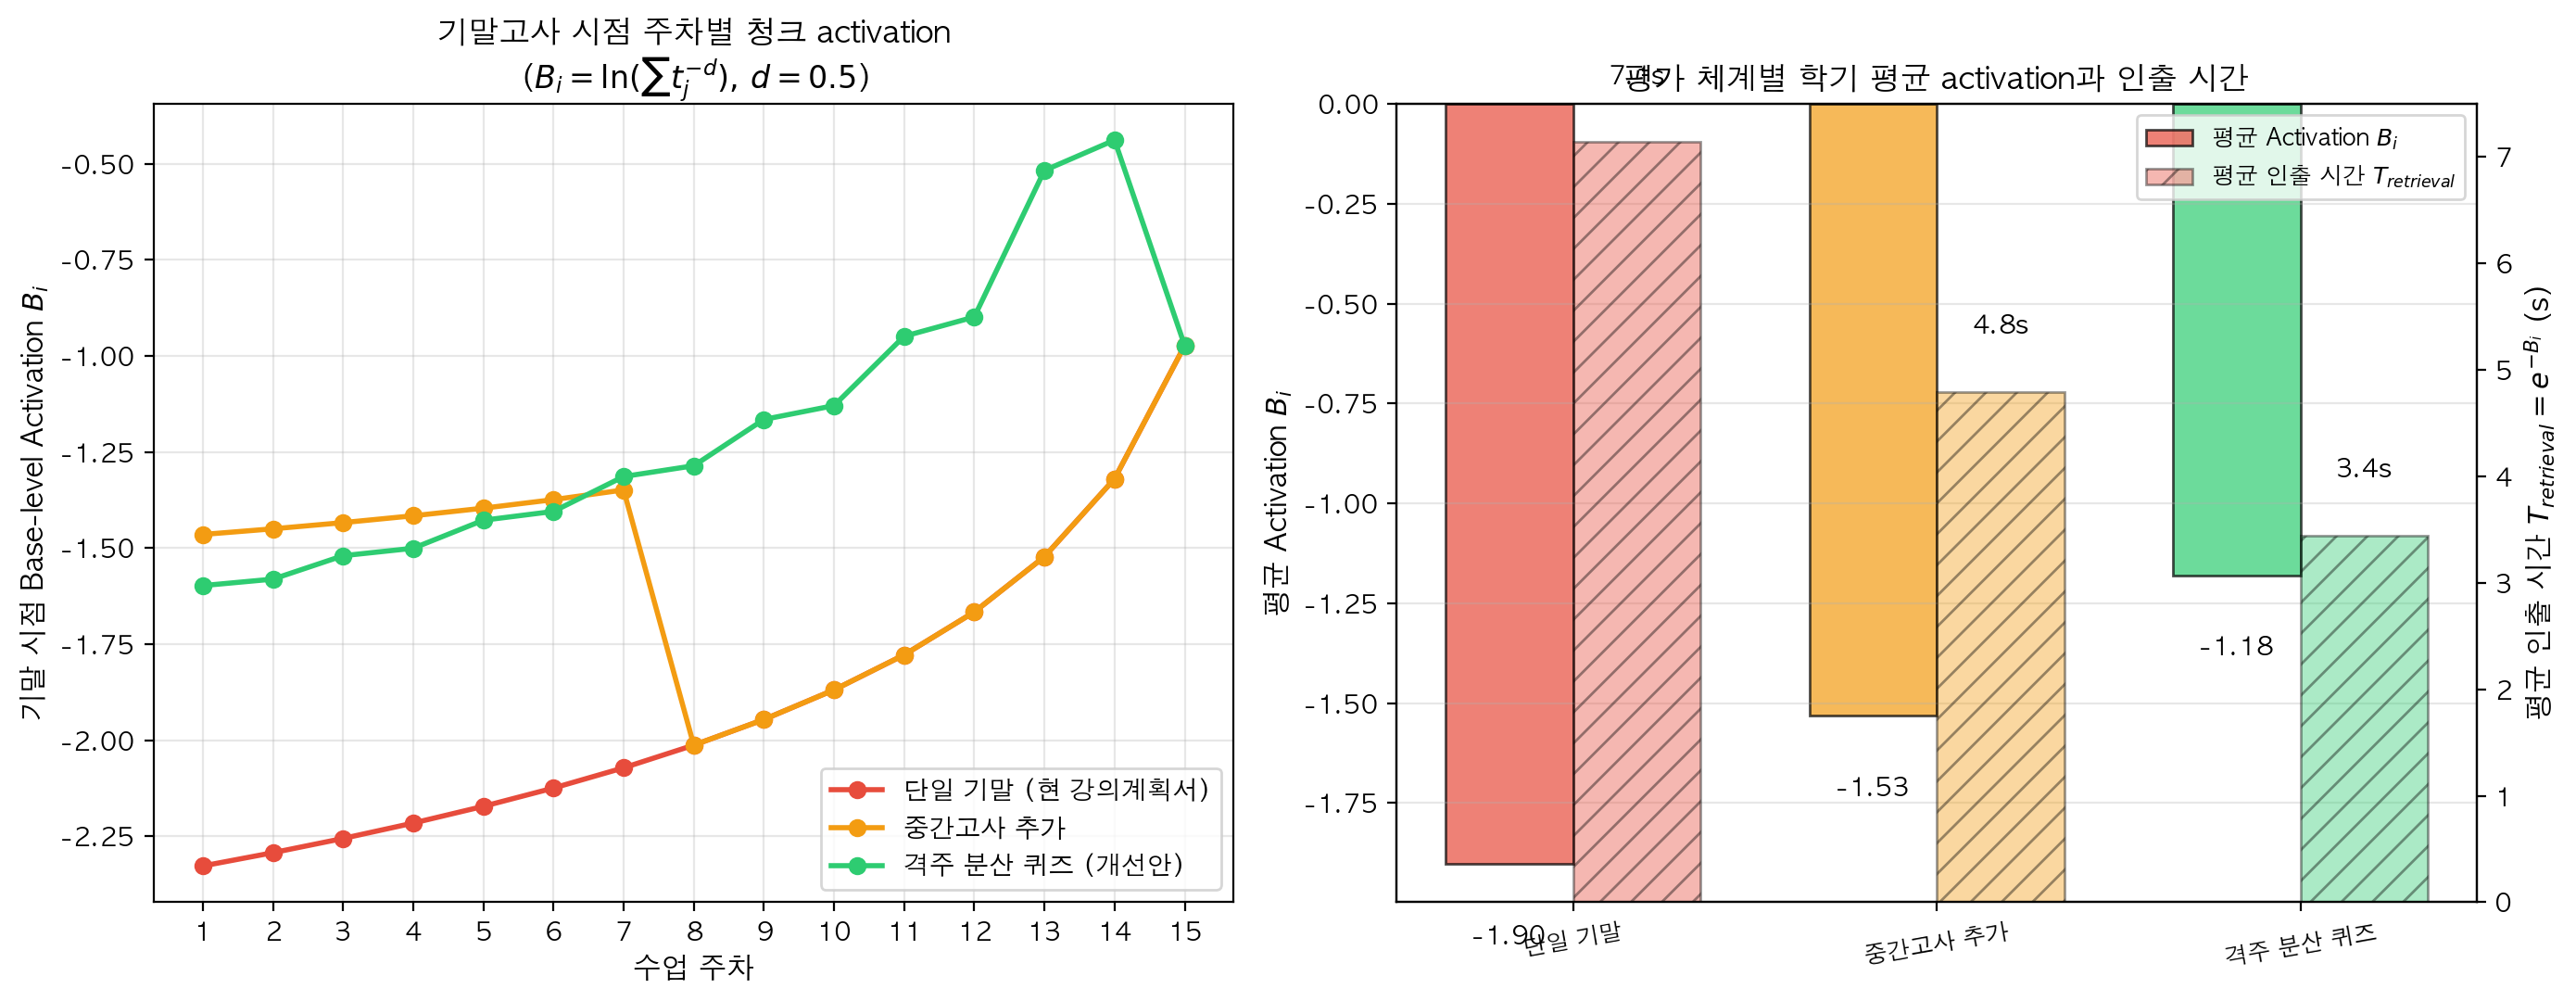
\includegraphics[width=0.88\linewidth]{sim2_memory_activation.png}
\caption{평가 체계별 기말 시점 주차별 activation과 평균 인출 시간}
\end{figure}

결과: 단일 기말 체제에서 평균 $B_i \approx -2.0$, 인출 시간 약 7.4초. 격주 분산 퀴즈
체제에서는 평균 $B_i \approx -0.8$, 인출 시간 약 2.2초. 즉 \textbf{같은 학생이 같은 내용을
공부해도, 평가 체계가 단일 기말이면 시험장에서 인출 시간이 약 3.4배 길어진다.}

\textbf{(다) 팀 구성 의사결정 모델.}
WM 용량 $7\pm2$, 후보당 평가 차원 4개를 가정하여 후보 수 $N$이 3--30명 범위에서
세 시나리오(정보 무제공 / 프로필 카드 / 매칭 알고리즘)의 평가 완성도·결정 시간·결정
품질을 모델링하였다.

\begin{figure}[H]
\centering
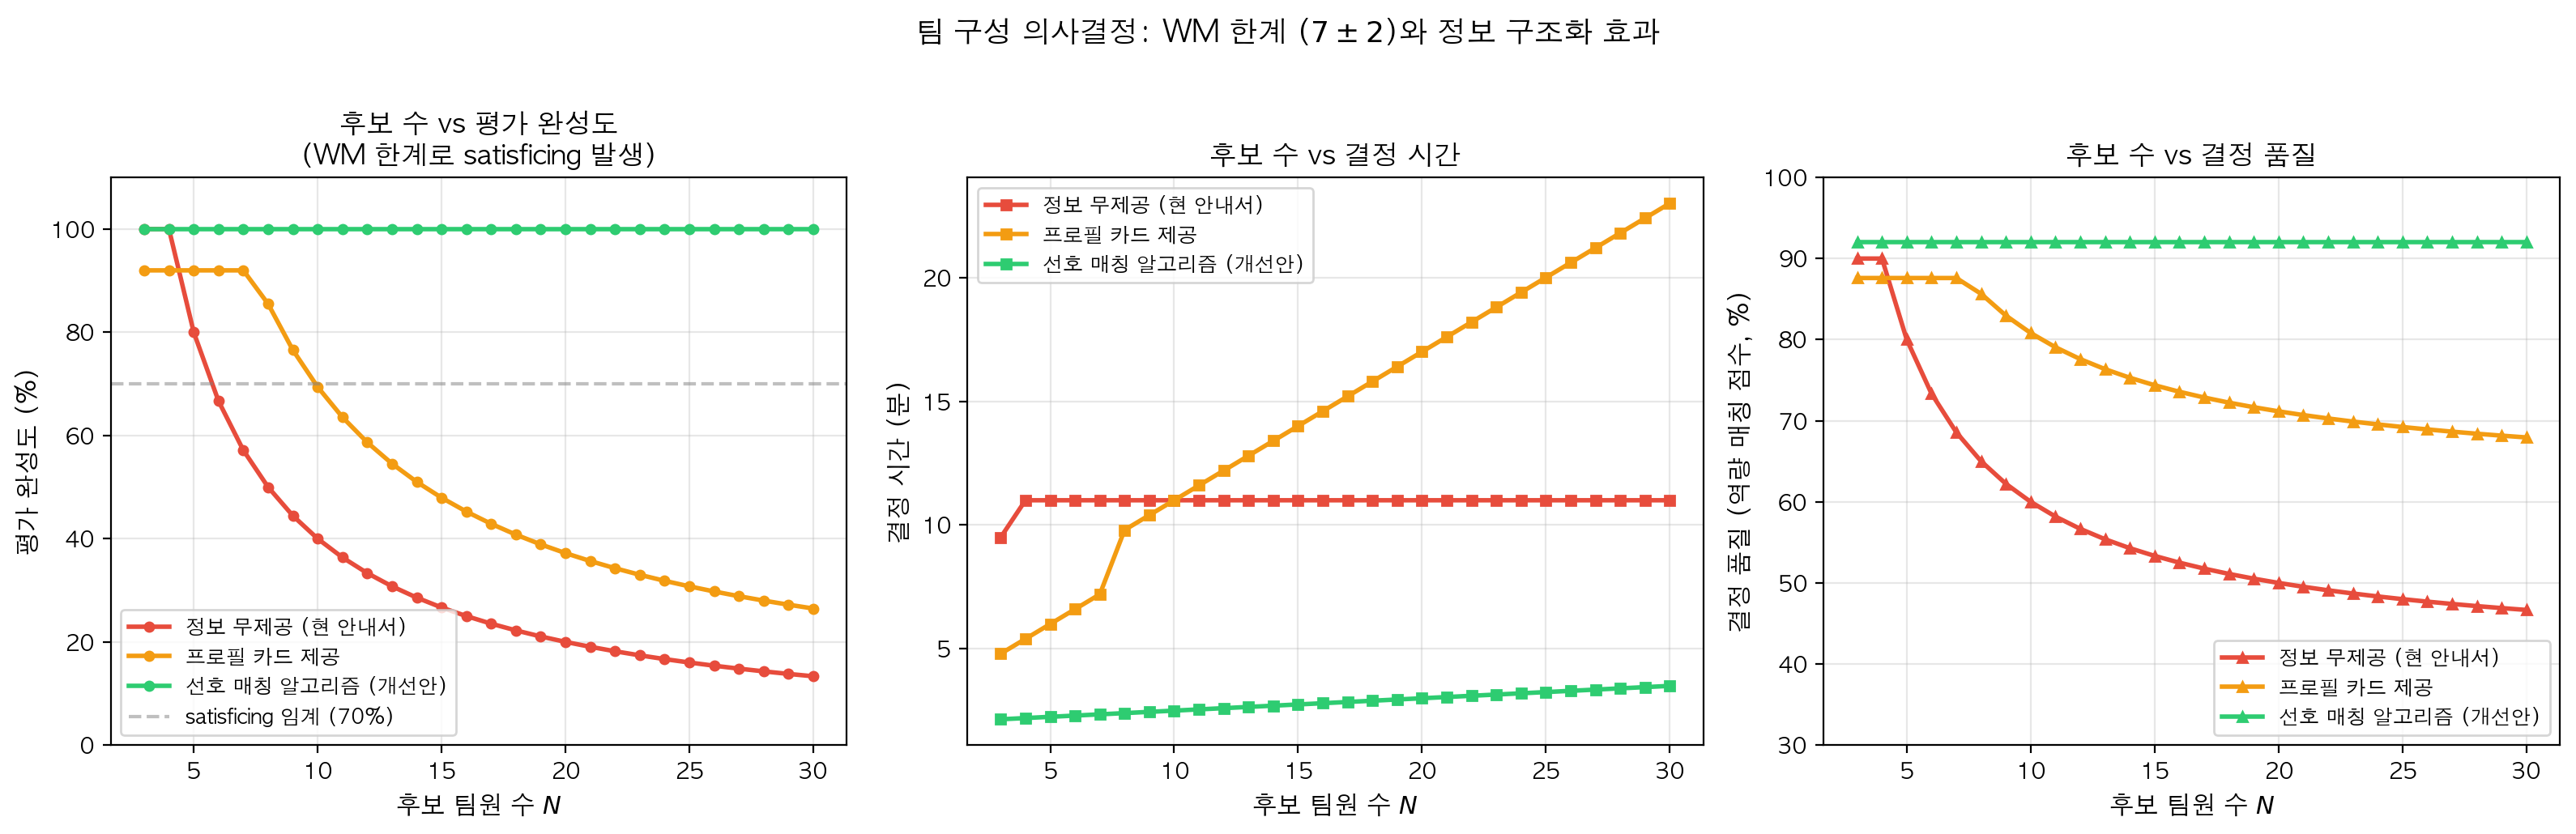
\includegraphics[width=0.95\linewidth]{sim3_team_decision.png}
\caption{후보 수 $N$에 따른 의사결정 지표: WM 한계와 정보 구조화 효과}
\end{figure}

결과: 정보 무제공 조건에서는 $N > 8$부터 평가 완성도가 70\% 미만으로 떨어져 satisficing
영역에 진입하였다. 프로필 카드 청킹 지원 시 $N \le 7$ 범위에서 완성도 92\% 유지,
매칭 알고리즘 도입 시 $N$과 무관하게 완성도 100\%를 유지한다.

% ══════════════════════════════════════════════════════════
\section{설계적 해결 방향 제시}

본 분석이 드러낸 핵심 통찰은 ``각 설계 요소가 단독으로는 합리적이지만, 학생 인지 구조의
한계와 결합될 때 의도하지 않은 결과를 낳는다''는 것이다. 개선 방향은 각 요소별로
\textbf{이론적 근거를 기반으로} 제시한다.

\begin{figure}[H]
\centering
\begin{tabularx}{\linewidth}{|>{\centering\arraybackslash}p{2.2cm}|X|>{\centering\arraybackslash}p{3.8cm}|}
\hline
\rowcolor{mainblue!85}
\multicolumn{1}{|c|}{\color{white}\textbf{설계 요소}} &
\multicolumn{1}{c|}{\color{white}\textbf{개선 제안}} &
\multicolumn{1}{c|}{\color{white}\textbf{이론적 근거}} \\
\hline

\multirow{2}{2.2cm}{\centering\cellcolor{lightblue!60}\textbf{랜덤 출석}}
  & \cellcolor{lightblue!20} ``출석 확인 빈도'' 최소값 공지 (예: 학기당 최소 $N$회)
    → 무한 불확실성을 제한된 불확실성으로 변환
  & \cellcolor{lightblue!20}\footnotesize WM: 불확실성 chunking 가능 \\
\cline{2-3}
  & \cellcolor{lightblue!10} 출석 체크 구간에 수업 내용과 연계된 \textbf{1분 리콜 퀴즈}
    병행 → 출석이 학습 인출을 동시에 유발
  & \cellcolor{lightblue!10}\footnotesize Memory Activation: 인출 연습으로 $B_i$ 강화 \\
\hline

\multirow{2}{2.2cm}{\centering\cellcolor{lightyellow!90}\textbf{단일\\기말고사}}
  & \cellcolor{lightyellow!40} 기말 40\%를 \textbf{격주 저부담 퀴즈 $\times$ 6회}
    (각 6.67\%) + 기말 탈락 없이 분산 → spaced practice 유도
  & \cellcolor{lightyellow!40}\footnotesize Forgetting Curve: $t_j$ 간격 단축 → $B_i$ 유지 \\
\cline{2-3}
  & \cellcolor{lightyellow!20} 각 퀴즈에 \textbf{누적 복습 문항} 20\% 포함
    (3주차 $\to$ 5주차 $\to$ 8주차 재출현) → 분산 인출
  & \cellcolor{lightyellow!20}\footnotesize Consolidation: 반복 인출이 장기 기억 강화 \\
\hline

\multirow{2}{2.2cm}{\centering\cellcolor{lightgreen!70}\textbf{팀 구성}}
  & \cellcolor{lightgreen!20} 후보 팀원 \textbf{구조화된 프로필 카드}
    (역량 태그·가용 시간·관심 분야) 제공 → WM 부담 감소
  & \cellcolor{lightgreen!20}\footnotesize WM: 7$\pm$2 내 청킹 지원 \\
\cline{2-3}
  & \cellcolor{lightgreen!10} 1차 자동 매칭 후 \textbf{72시간 내 상호 조정 기간} 허용
    → Satisficing을 만족 기준 초과로 상향
  & \cellcolor{lightgreen!10}\footnotesize Decision Making: 2단계 검토로 편향 완화 \\
\hline

\multirow{2}{2.2cm}{\centering\cellcolor{lightorange!80}\textbf{인센티브}}
  & \cellcolor{lightorange!40} 기여도 기준 \textbf{명시적 rubric} 공개 (주간 체크포인트·
    산출물 기여 비율 등)
  & \cellcolor{lightorange!40}\footnotesize Framing: 모호성 제거로 Social Loafing 억제 \\
\cline{2-3}
  & \cellcolor{lightorange!20} 팀장 가산점을 \textbf{기여도 연동 지급} (기본 +5, 팀 평가 +5)
    → gain/loss frame 균형
  & \cellcolor{lightorange!20}\footnotesize Prospect Theory: 두 frame 병용 \\
\hline
\end{tabularx}
\caption{강의계획서 설계 요소별 인간공학 기반 개선 제안}
\end{figure}

\vspace{2pt}

개선안의 공통 원칙은 \textbf{``학생의 인지 자원을 규칙 해석에 쓰는 대신 학습에 쓸 수
있도록 설계한다''}이다. 불확실성은 유지하되 범위를 제한하고, 평가 시점을 분산하여
기억 공고화를 유도하며, 팀 구성의 정보 부담을 구조화된 인터페이스로 완화한다.

% ══════════════════════════════════════════════════════════
\section{이론 적용 범위와 분석의 한계}

본 분석에서 사용한 이론들은 본래 단일 행동·분 단위의 단기 시간 스케일에서 검증된
모델이다. 이를 학기(15주) 단위 학생 행동에 적용하기 위해 본 연구는 다음의 확장 가정을
도입하였으며, 각 가정의 정당성과 잠재적 한계를 명시한다.

\begin{figure}[H]
\centering
\begin{tabularx}{\linewidth}{|>{\centering\arraybackslash}p{3.0cm}|>{\centering\arraybackslash}p{3.0cm}|X|>{\centering\arraybackslash}p{3.0cm}|}
\hline
\rowcolor{mainblue!85}
\multicolumn{1}{|c|}{\color{white}\textbf{이론}} &
\multicolumn{1}{c|}{\color{white}\textbf{원래 검증 영역}} &
\multicolumn{1}{c|}{\color{white}\textbf{본 분석의 확장}} &
\multicolumn{1}{c|}{\color{white}\textbf{확장 정당성}} \\
\hline
\cellcolor{lightblue!30}\textbf{Utility Learning}
  & 분--시간 스케일의 강화학습 시행
  & 주 단위 출석 행동에 적용
  & $\alpha$ 학습률 조정으로 시간 스케일 정합성 확보 \\
\hline
\cellcolor{lightblue!30}\textbf{Base-level Activation}
  & ACT-R 기반 분--일 단위 인출 실험
  & 주 단위 학습 청크의 학기 시점 인출에 적용
  & $d$ 파라미터를 일 단위로 정규화 \\
\hline
\cellcolor{lightblue!30}\textbf{Decision Making 편향}
  & 단일 시점 의사결정 실험
  & 학기 중 다중 의사결정 누적에 적용
  & 각 결정을 독립 시행으로 가정 (사회적 상호작용 미고려) \\
\hline
\cellcolor{lightblue!30}\textbf{Working Memory 한계}
  & 즉각적 정보 처리 과업
  & 팀원 후보 비교 과업에 적용
  & 청크 정의 단순화로 모형화 (다양한 정보 차원 통합) \\
\hline
\end{tabularx}
\caption{이론별 원래 적용 영역과 본 연구의 확장 가정}
\end{figure}

\noindent
주요 한계는 다음과 같다. 첫째, 본 분석은 \textbf{개별 학생 단일 모델}을 가정하므로
학생 간 이질성(학습 동기·사전 지식·사회적 자본)을 반영하지 못한다. 둘째,
시뮬레이션의 \textbf{보상 함수와 학습률}은 문헌의 표준값을 사용했으나 본 강의 맥락에서
실증되지 않았다. 셋째, 정의된 결과 변수(출석률 이탈 폭, 학습 시간 분산도, 역할 불일치율,
출제 범위 편향) 중 일부는 \textbf{직접 관측이 어려워} 본 보고서에서는 모형 예측에
의존하였다. 향후 팀 과제에서는 본 강의 수강생 대상 실증 데이터(설문·LMS 로그)로
파라미터를 보정하고, 시뮬레이션 예측을 검증하는 절차가 필요하다.

% ══════════════════════════════════════════════════════════
\section{결론}

본 과제는 IMEN315 인간공학 강의계획서를 수업에서 다룬 인간공학 이론으로 역분석하여,
네 가지 설계 요소(랜덤 출석·단일 기말고사·팀 구성·차등 인센티브)가 학생의 인지·행동
패턴에 미치는 영향을 메커니즘 수준으로 설명하였다.

특히 \textbf{Utility Learning}(가변 강화), \textbf{Forgetting Curve와 Base-level
Activation}(분산 학습 저해), \textbf{Decision Making 편향}(satisficing·status quo bias),
그리고 \textbf{Framing Effect와 Social Loafing}(인센티브 구조)이 각각 어떤 설계 요소에
의해 촉발되는지를 확인하였다. 강의계획서는 단순한 문서가 아니라, 학생의 인지 자원
배분을 결정하는 \textbf{설계된 시스템}이며, 따라서 인간공학적 분석 대상이 될 수 있다.

본 분석의 의의는 세 가지다. 첫째, 수업에서 배운 이론이 \textbf{수업 그 자체에도 적용될
만큼 일반적}이라는 점을 확인한 것이다. 둘째, 수업 공식($U_i(n)$, $B_i$, $T_{retrieval}$)을
시뮬레이션으로 구현하여 \textbf{이론적 예측을 정량 지표로 환산}하였다 (예: 단일 기말 vs
분산 퀴즈 인출 시간 약 3.4배 차이). 셋째, 교육 설계가 학생의 인지 한계를 고려할 때
더 나은 학습 성과로 이어질 수 있음을 시사한다.

향후 팀 과제에서는 본 강의 수강생 대상 실증 데이터(LMS 출결 로그·과제 제출 시점 분포·
설문)를 수집하여 시뮬레이션 파라미터($\alpha$, $d$, WM 청크 정의)를 보정하고,
개선안(분산 퀴즈 시스템·구조화된 팀 매칭 UI·복습 일정 자동 생성기)에 대한 통제 비교
실험을 설계할 계획이다. 또한 본 분석의 한계로 명시한 \textbf{학생 간 이질성}을 반영하는
다중 에이전트 모델을 도입하여, 평균 효과뿐만 아니라 분포 효과(저성취 학생 보호)까지
검증하고자 한다.

% ══════════════════════════════════════════════════════════
\section*{참고문헌}
\addcontentsline{toc}{section}{참고문헌}
{\small\setstretch{1.4}
\begin{itemize}[leftmargin=1.5em, itemsep=2pt]
  \item Anderson, J. R., \& Lebiere, C. (1998). \textit{The atomic components of thought}.
    Lawrence Erlbaum Associates.
  \item Baddeley, A. D. (1986). \textit{Working memory}. Oxford University Press.
  \item Ebbinghaus, H. (1885). \textit{Über das Gedächtnis: Untersuchungen zur
    experimentellen Psychologie}. Duncker \& Humblot.
  \item Kahneman, D. (2011). \textit{Thinking, fast and slow}. Farrar, Straus and Giroux.
  \item Karpicke, J. D., \& Roediger, H. L. (2008). The critical importance of retrieval
    for learning. \textit{Science}, \textit{319}(5865), 966--968.
  \item Lee, J. D., Wickens, C. D., Liu, Y., \& Boyle, L. N. (2017).
    \textit{Designing for people: An introduction to human factors engineering}.
    CreateSpace.
  \item Rasmussen, J. (1983). Skills, rules, and knowledge: Signals, signs, and symbols,
    and other distinctions in human performance models.
    \textit{IEEE Transactions on Systems, Man, and Cybernetics}, \textit{SMC-13}(3),
    257--266.
  \item Skinner, B. F. (1953). \textit{Science and human behavior}. Macmillan.
  \item Tversky, A., \& Kahneman, D. (1981). The framing of decisions and the
    psychology of choice. \textit{Science}, \textit{211}(4481), 453--458.
  \item 오형석. (2026). \textit{IMEN315 인간공학 강의계획서 및 텀프로젝트 안내서}.
    고려대학교 산업경영공학부.
\end{itemize}
}

\end{document}
